\documentclass{standalone}

\begin{document}


\section*{Mathematical background}\addcontentsline{toc}{section}{Mathematical background}
\markboth{Appendix A}{Mathematical background}

Since the exact knowledge of the prior probabilities and conditional probabilities is possible only on theory a parametric approach is often needed.
A parametric approach aim to create reasonable hypothesis about the distribution under analysis and its fundamental parameters (e.g mean and variance).
In the next of this discussion we focused only on normal distributions for convenience.

Given the multi-dimensional form of Gauss distribution:

$$
G(\mathbf{x}|\mu, \Sigma) = \frac{1}{(2\pi)^{d/2}\cdot\left|\Sigma\right|^{1/2}}\cdot exp\left[-\frac{1}{2}(\mathbf{x}-\mathbf{\mu})^T\Sigma^{-1}(\mathbf{x}-\mathbf{\mu})\right]
$$
\\
where $\mathbf{x}$ is a column $d$-dimensional vector, $\mathbf{\mu}$ the mean vector of the distribution, $\Sigma$ the covariance matrix ($d\times d$), $|\Sigma|$ and $\Sigma^{-1}$ the determinant and the inverse of $\Sigma$, respectively, we can notice the $G$ depends quadratically by $\mathbf{x}$,

$$
\Delta^2 = (\mathbf{x}-\mu)^T\Sigma^{-1}(\mathbf{x}-\mu)
$$
\\
where the exponent ($\Delta^2$) is called Mahalanobis distance of vector $\mathbf{x}$ from its mean.
This distance can be reduced to the Euclidean distance when the covariance matrix is the identity $\mathbf{I}$.

The covariance matrix is always symmetric and positive semi-definite (useful information for next algorithmic strategies) so it has an inverse.
If the covariance matrix has only diagonal terms the multidimensional distribution can be express as simple product of $d$ mono-dimensional normal distributions.
In this case the main axes are parallel to the Cartesian axes.

Starting from the multi-variate Gaussian distribution expression\footnote{
  In Machine Learning it will correspond to the conditional probability density.
}, the Bayesian rule for classification problems can be rewrite as:

$$
g_i(\mathbf{x}) = P(w_i|\mathbf{x}) = \frac{p(\mathbf{x}|w_i)P(w_i)}{p(\mathbf{x})} = \frac{1}{(2\pi)^{d/2}\cdot\left|\Sigma_i\right|^{1/2}}\cdot exp\left[-\frac{1}{2}(\mathbf{x}-\mathbf{\mu_i})^T{\Sigma_i}^{-1}(\mathbf{x}-\mathbf{\mu_i})\right] \frac{P(w_i)}{p(\mathbf{x})}
$$
\\
where, removing constant terms ($\pi$ factors and absolute probability density $p(\mathbf{x}) = \sum_{i=1}^s p(\mathbf{x}|w_i)\cdot P(w_i)$) and using the monotonicity of the function, we can extract the logarithmic relation:

$$
g_i(\mathbf{x}) = -\frac{1}{2}(\mathbf{x}-\mu_i)^T{\Sigma_i}^{-1}(\mathbf{x}-\mu_i) -\frac{1}{2}\log\left|\Sigma_i\right|+\log P(w_i)
$$
\\
which is called Quadratic Discriminant function.

The function dependency by the covariance matrix allows 5 different cases:

\begin{itemize}

\item \textbf{$\Sigma_i=\sigma^2I$ - DiagLinear Classifier}

\begin{minipage}{.30\textwidth}
\hspace{-.5cm}
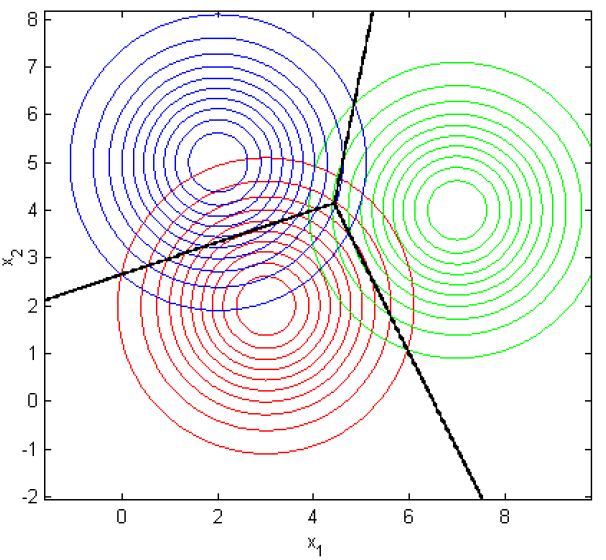
\includegraphics[width=1\textwidth]{case1.png}
\end{minipage}%
\begin{minipage}{.70\textwidth}
This is the case of completely independence of features, where they have equal variance for each class.
This hypothesis allow us to simplify the discriminant function as:
\end{minipage}\\

$$
g_i(\mathbf{x})=-\frac{1}{2\sigma^2}(\mathbf{x^Tx}-2{\mu_i}^T\mathbf{x} + {\mu_i}^T\mu_i) + \log P(w_i)
$$
\\
and removing all the $\mathbf{x^Tx}$ constant terms for each class

$$
g_i(\mathbf{x}) = -\frac{1}{2\sigma^2}(-2{\mu_i}^T\mathbf{x}+{\mu_i}^T\mu_i)+\log P(w_i) = \mathbf{{w_i}^Tx}+\mathbf{w_0}
$$
\\
This simplifications create a linear discriminant function where the separation surfaces between classes are hyper-planes ($g_i(\mathbf{x})=g_j(\mathbf{x})$).

With equal prior probability the function can be rewritten as

$$
g_i(\mathbf{x}) = -\frac{1}{2\sigma^2}(\mathbf{x}-\mu_i)^T(\mathbf{x}-\mu_i)
$$
\\
which is called \emph{nearest mean classifier} where the equal-probability surfaces are hyper-spheres.


\item \textbf{$\Sigma_i = \Sigma$ (diagonal matrix) - Linear Classifier}

\begin{minipage}{.30\textwidth}
\hspace{-.5cm}
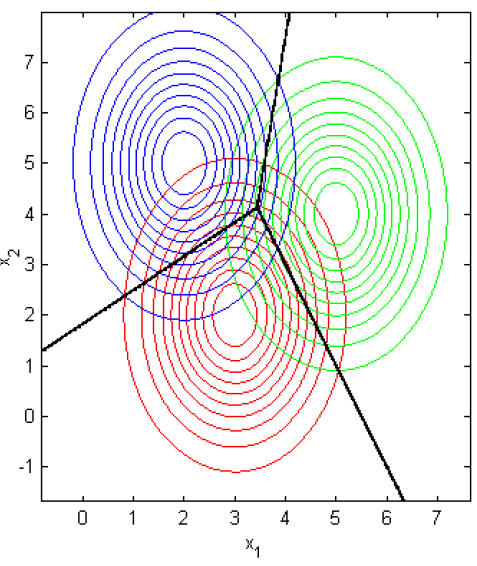
\includegraphics[width=1\textwidth]{case2.png}
\end{minipage}%
\begin{minipage}{.70\textwidth}
In this case the classes have same covariances but each feature has its own different variance.
After the $\Sigma$ substitution in the equation, we obtain
\end{minipage}\\

$$
g_i(\mathbf{x}) = -\frac{1}{2}\sum_{k=1}^{s}\frac{(\mathbf{x_k}-\mu_{i,k})^2}{{\sigma_k}^2}-\frac{1}{2}\log\prod_{k=1}^{s}{\sigma_k}^2+\log P(w_i)
$$
\\
where we can remove constant $\mathbf{x_k}^2$ terms (equals for each class) and obtain another time a linear discriminant function where the discriminant surfaces are hyper-planes and equal-probability boundaries given by hyper-ellipsoids.
Note that the only difference from the previous case is the normalization factor of each axes that in this case is given by the its variance.


\item \textbf{$\Sigma_i = \Sigma$ (non-diagonal matrix) - Mahalanobis Classifier}

\begin{minipage}{.30\textwidth}
\hspace{-.5cm}
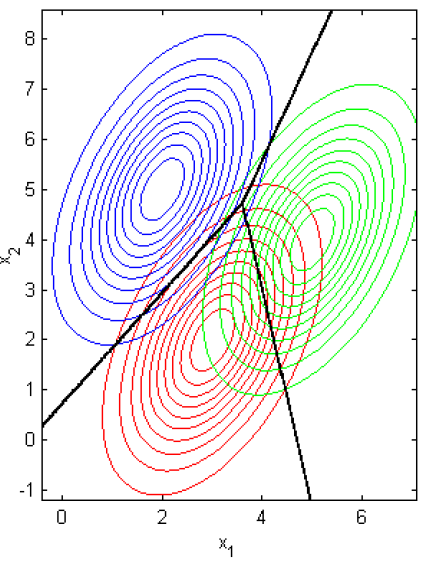
\includegraphics[width=1\textwidth]{case3.png}
\end{minipage}%
\begin{minipage}{.70\textwidth}
In this case we assume that each class has the same covariance matrix but they are non-diagonal ones.
The discriminant function becomes
\end{minipage}\\

$$
g_i(\mathbf{x}) = -\frac{1}{2}(\mathbf{x}-\mu_i)^T{\Sigma}^{-1}(\mathbf{x}-\mu_i) -\frac{1}{2}\log\left|\Sigma\right|+\log P(w_i)
$$
\\
where we can remove the $\log\left|\Sigma\right|$ term because it is constant for all the classes and we can assume equal prior probability.
In this case we obtain

$$
g_i(\mathbf{x}) = -\frac{1}{2}(\mathbf{x}-\mu_i)^T{\Sigma}^{-1}(\mathbf{x}-\mu_i)
$$
\\
where the quadratic term is the Mahalanobis distance, i.e a normalization of the distance according to the inverse of their covariance matrix.
We can prove that expanding the scalar product and removing the constant term $\mathbf{x^T\Sigma^{-1}x}$, we obtain yet a linear discriminant function with the same properties of the previous case.
In this case the hyper-ellipsoids have axes aligned according to the eigenvectors of the $\Sigma$ matrix.


\item \textbf{$\Sigma_i = {\sigma_i}^2I$ - DiagQuadratic Classifier}

\begin{minipage}{.30\textwidth}
\hspace{-.5cm}
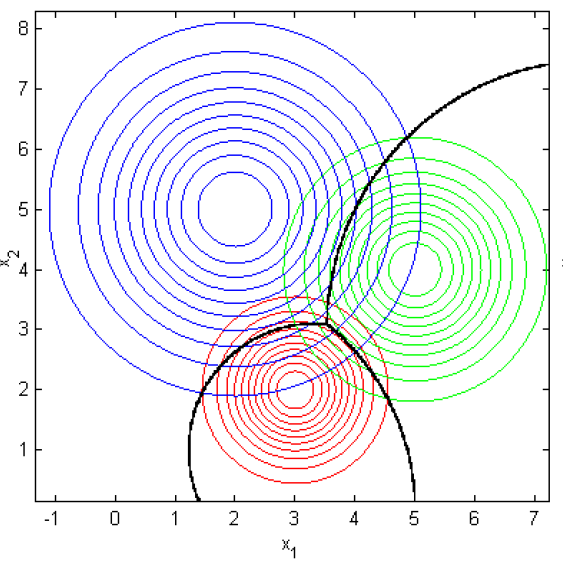
\includegraphics[width=1\textwidth]{case4.png}
\end{minipage}%
\begin{minipage}{.70\textwidth}
In this case we have different covariance matrix for each class but they are proportional to the identity matrix, i.e diagonal matrix.
The discriminant function in this case becomes
\end{minipage}\\

$$
g_i(\mathbf{x}) = -\frac{1}{2}(\mathbf{x}-\mu_i)^T{\sigma_i}^{-2}(\mathbf{x}-\mu_i) -\frac{1}{2}s\log\left|{\sigma_i}^2\right|+\log P(w_i)
$$
\\
where this expression can be further reduced obtaining a quadratic discriminant function.
In this case the equal-probability boundaries are hyper-spheres aligned according to the feature axes.


\item \textbf{$\Sigma_i \neq\Sigma_j$ (general case) - Quadratic Classifier}

\begin{minipage}{.30\textwidth}
\hspace{-.5cm}
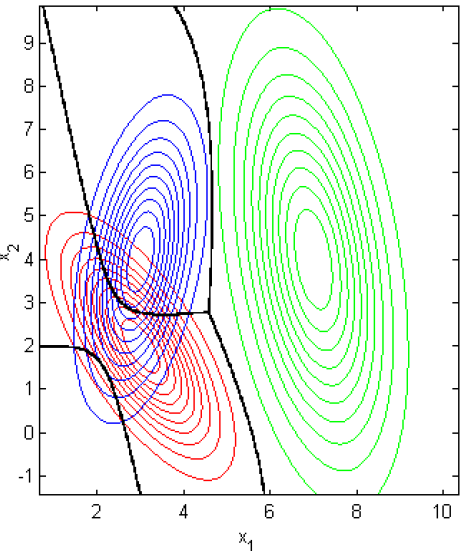
\includegraphics[width=1\textwidth]{case5.png}
\end{minipage}%
\begin{minipage}{.70\textwidth}
Starting from the more general discriminant function we can relabel the variables and highlight its quadratic form as
\end{minipage}\\

$$
g_i(\mathbf{x}) = \mathbf{x^TW_{2,i}x}+\mathbf{w_{1,i}^Tx} + \mathbf{w_{0,i}} \quad \mbox{with}\quad \left\{\begin{array}{l} \mathbf{W_{2,i}}=-\frac{1}{2}{\Sigma_i}^{-1}\\ \mathbf{w_{1,i}}={\Sigma_i}^{-1}\mu_i \\ \mathbf{w_{0,i}}=-\frac{1}{2}{\mu_i}^T{\Sigma_i}^{-1}\mu_i-\frac{1}{2}\log\left|\Sigma_i\right|+\log P(w_i) \\ \end{array}\right.
$$
\\
In this case each class has its own covariance matrix $\Sigma_i$ and the equal-probability boundaries are hyper-ellipsoids oriented according to the eigenvectors of the covariance matrix of each class.

\end{itemize}

The Gaussianity of dataset distribution should be tested before using this classifiers.
It can be performed using statistical tests as \href{https://www.jstor.org/stable/2284163?seq=1#page_scan_tab_contents}{\emph{Malkovich-Afifi}} based on \href{https://en.wikipedia.org/wiki/Kolmogorov–Smirnov_test}{\emph{Kolmogorov-Smirnov}} index or just simpler with the empirical visualization of the data points.


\end{document}
